%
% Copyright (c) 2020 Antonio Coín Castro
%
% This work is licensed under a
% Creative Commons Attribution-ShareAlike 4.0 International License.
%
% You should have received a copy of the license along with this
% work. If not, see <http://creativecommons.org/licenses/by-sa/4.0/>.

In this chapter we will concentrate on the design and implementation of several fuzzy systems for working with Big Data. While approaching these systems from a theoretical perspective as we have been doing throughout the text, we will shift our focus somewhat and also describe a number of implementations in an actual programming language. This part can be regarded as a more practical aspect of our work, a small software development project undertaken with the intent of fusing the ideas previously presented.

The language of choice is the Scala programming language, and the platform to develop our Big Data programs will be no other than Apache Spark. Although we will generally provide a high-level description of the algorithms, we will also insert occasional pieces of code that help clarify what we are trying to achieve, and even sometimes discuss technical aspects of the implementation or particularities of the language.

The interested reader can refer to \cite{suereth2012scala} or \cite{odersky2008programming} for a detailed introduction to Scala. Basic and intermediate notions of the interaction between Scala and Spark are also covered in \cite{karau2015learning}.

\section{Learning algorithms for fuzzy systems}

There are basically two different strategies to build FRBS, depending on the information available at the moment of its construction. The first way is to rely on human experts, inputting the knowledge manually into the system. This is one of the main tasks tackled in the field of \textit{knowledge engineering}, where knowledge engineers devise the best methods to extract and properly represent the knowledge from experts in the matter. The other way is to try to learn the rules and behaviour of the system from the data, by using several learning methods. We will concentrate on the latter approach.

Generally speaking, learning algorithms for FRBSs can be decomposed in two stages: a structure identification step and a parameter tuning phase. In the first one, the structure and size of the rule base is estimated, while in the second one the parameters corresponding to the various membership functions involved are optimized. These steps can be performed sequentially or in a simultaneous way.

While these algorithms are tailored to work with fuzzy systems, the restrictions and particularities of the general learning algorithms still apply. That is, choosing a specific algorithm is only one step of the full learning process: data preprocessing, dimensionality reduction, parameter selection, etc. A number of software libraries have been developed to work with fuzzy systems, among which we would like to highlight the \verb|frbs| R package \cite{riza2015frbs}. It gathers a multitude of classification and regression algorithms under a common API that focuses on easiness of use.

Before we specify the algorithms implemented, we present an overview of the three main types of learning algorithms for FRBSs.

\subsection{Space partition algorithms}

These algorithms are designed so that a partition on the input and output spaces is established, and rules are derived from the grade in which each data point represents each of these partitions. In other words, rules are created \textit{ad-hoc} directly from the data.

The parameters of the membership functions are dependent on the specific technique used to partition the spaces, and the expressions used to measure the affinity of each point to each partition. A notable special case is the use of \textit{clustering algorithms} to make the partitions. Generally speaking, the purpose of clustering is to group together data points that share certain features, with the hope of detecting similarities and obtaining a more concise representation of a system's behaviour, which we can later use to refine it. In this case, each centroid acts as a fuzzy rule, with a membership function that measures the grade in which each points belongs to each centroid. This is known as \textit{fuzzy clustering}, and differs from classical clustering algorithms in that each point generally belongs to every cluster to a greater or lesser extent, not just to one of them.

\subsection{Neural network algorithms}

As their name indicates, these algorithms are based on the concept of artificial neural networks. These structures have been adapted from the field of machine learning and more precisely of deep learning, where they are widely used and serve as the basis of multiple state of the art algorithms (see for example \cite{lecun2015deep}).

The FRBS is usually generated beforehand, and it is then adapted to fit a neural network structure. This network is used as a way of tuning the parameters of the membership function using the backpropagation algorithm, and thus retaining all the advantages of this technique. A typical neuro-fuzzy system has a layer that represents the membership functions of the linguistic values associated with the input variables, an antecedent layer that represents the antecedent parts of every rule, a consequent layer to express the consequent of the rules, and a defuzzification layer to provide a final response. Commonly there are weights involved in the process that calibrate the importance of each rule, and they can also be adjusted when training the network. A good example of this type of algorithm is the HyFIS algorithm \cite{kasabov1999hyfis}, which uses a 5-layer neural network structure and a hybrid learning scheme.

\subsection{Genetic algorithms}

We arrive at the last type of FRBS considered here, which is based on genetic algorithms. Ample research has been conducted on this topic, and the reader can refer to \cite{cordon2011historical} for a historical review or to \cite{cordon2001genetic} for a whole book on the subject.

The philosophy behind these algorithms is similar to that of the neuro-fuzzy systems: an initial structure is established, and then a genetic method is adapted to tune a specified set of parameters. But genetic algorithms can also be used to generate the whole structure from the start, as shown in \cite{cordon2001generating}. As an alternative to neuro-fuzzy systems, these algorithms present all the advantages (as well as the disadvantages) of the standard genetic methods. We mention a couple of them that are studied in the literature.

\begin{enumerate}[1.]
  \item The first one is a basic genetic fuzzy system based on Thrift's method \cite{thrift1991genetic} of integer coding. In this method, which follows an elitist scheme, each possible rule represents a chromosome, and a new population is obtained by applying the usual crossover and mutation operators (although mutations are adapted to this particular setting). The fitness of an individual is calculated as the mean squared error between predictions and actual values, as output by the system.
  \item Cordón and Herrera proposed the D-MOGUL method \cite{cordon1997three} to automatically generate a complete knowledge base; it uses a genetic algorithm to determine the structure of the fuzzy rules and the parameters of the membership functions simultaneously. It consists on three steps:
  \begin{itemize}
    \item An iterative \textit{rule generation} process that explores the search space for rules that satisfy certain desirable conditions. A partition of the input space consisting on triangular membership functions is considered.
    \item A \textit{genetic simplification phase}, that eliminates redundant rules from the previous step by exploring the subsets of rules that best cooperate among themselves.
    \item A \textit{genetic tuning phase} in which membership parameters are adjusted to try to maximize the accuracy of the final model.
  \end{itemize}
\end{enumerate}

\section{Fuzzy learning algorithms implemented}

Before proceeding with the implementation tasks, and even before starting the theoretical study that we have already presented in the previous chapters, we made an estimation of the total cost of this project and the temporal planning involved, which can be consulted in Appendix \ref{app:planning}.

We begin with an implementation of a basic state partition algorithm, arguably the simplest one of its family, but one that will provide a starting point from which to build upon. We continue our implementation task with two algorithms that belong to the family of fuzzy clustering methods. As we will see shortly they are closely related, and the fact that neither of them was available in the MLlib library at the time of writing this thesis was enough motivation to implement both of them.

We tried to follow MLlib's code style and conventions as much as possible, though at some points there might be some deviations from said conventions, and a few adjustments would probably be needed in order to integrate these algorithms in the library. Nevertheless, the philosophy of building a model, fitting it to some data and then using it to make predictions is still there.

\subsection{Wang \& Mendel algorithm}

The first algorithm developed is the Wang \& Mendel algorithm for learning fuzzy rules from examples \cite{wang1992generating}, which as explained before is a basic space partition algorithm for fuzzy systems. In general terms, it divides the input and output spaces to make a grid, and uses these divisions to infer the rules of the system checking how well the data fits in each portion of the grid. Supposing that we have a collection of $n$ input-output pairs of the form $(x_1^{(1)}, x_2^{(2)}; y^{(1)}),\dots, (x_1^{(n)}, x_2^{(n)}; y^{(n)})$, we summarize below the principal steps of this algorithm (the extension to the multi-input multi-output case is straightforward).

In \textit{Step 1}, we assume that the domain intervals of the variables are $[x_1^-,x_1^+], [x_2^-,x_2^+]$ and $[y^-,y^+]$, which means that with high probability the data on each dimension will lie on those intervals. We then divide each interval in $2N+1$ regions ($N$ can be different for each variable), and assign a membership function to each region. In our implementation we have chosen triangular membership functions, but other choices such as trapezoidal and Gaussian are possible as well. Each region is may be given a name that represents our understanding of the intervals (for example, we could name them $S1,\dots, SN, C, B1, \dots, BN$, where `$S$' stands for small, `$C$' for center and `$B$' for big). A sample partition of the input and output spaces can be seen in Figure \ref{fig:wm}.

\begin{figure}[h!]
\centering
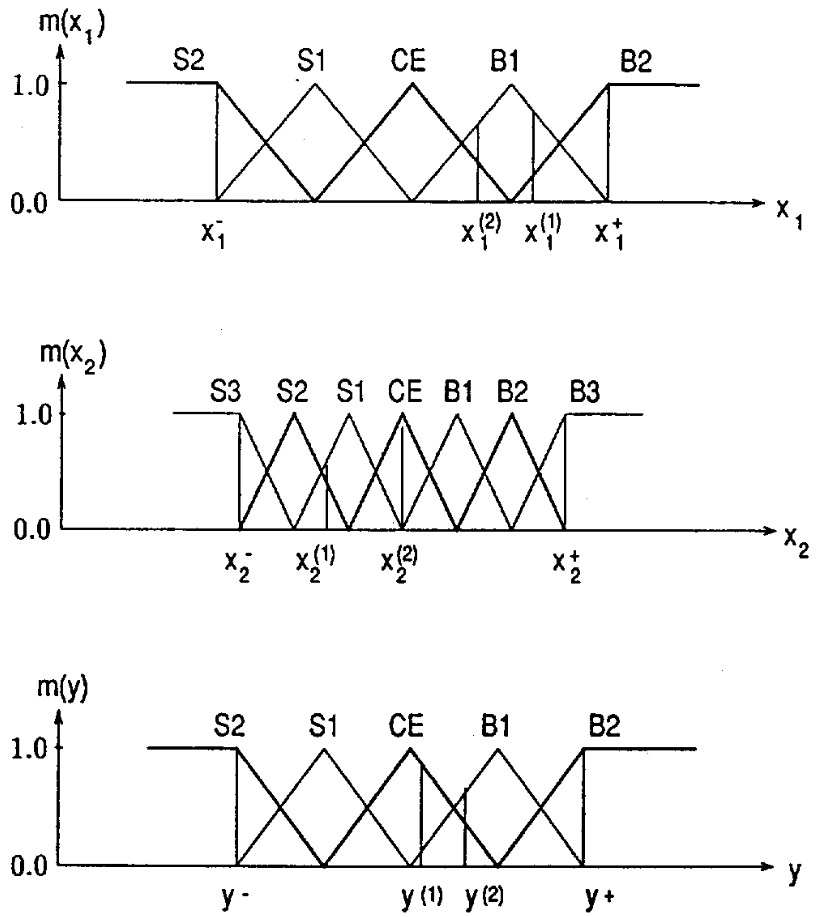
\includegraphics[width=.5\textwidth]{wm.jpg}
\caption{Sample division of input output spaces in fuzzy regions. Taken from \cite{wang1992generating}.}
\label{fig:wm}
\end{figure}

In \textit{Step 2}, we proceed to the generation of fuzzy rules based on the data points. For the $i$th data point, we compute the membership of $x_1^{(i)},x_2^{(i)}$ and $y^{(i)}$ to each of the regions in their respective dimension, and in each case we select the region with the highest membership. Then we form a rule in which the antecedents are the regions found in the input space, and the consequent is the region selected in the output space. For example, if the regions found were $S1$, $CE$ and $S1$, then the rule would look like
\begin{equation}\label{eq:rule}
  \text{if $x_1$ is $S1$ and $x_2$ is $CE$ then $y$ is $S1$}.
\end{equation}

In \textit{Step 3} we assign a degree of activation to each rule, which is simply the product of the values of the membership functions of the data point in question to each of the selected regions in each dimension. For example, if we take the rule shown in \eqref{eq:rule} its degree would be $D=m_{S1}(x_1)m_{CE}(x_2)m_{S1}(y)$.

In \textit{Step 4} we finally create a combined rule base, aggregating all the rules previously found. To prevent duplicates and conflicts, we only select among the rules with the same antecedent those which have the highest degree.

Finally, \textit{Step 5} is regarded as part of the prediction phase. For a given input $(x_1,x_2)$ we combine the antecedents of the $i$th fuzzy rule to determine the degree to which it is satisfied by $(x_1,x_2)$, and we denote it by
\[
m^i_{O^i} = m_{I_1^i}(x_1)m_{I_2^i}(x_2),
\]
where $O^i$ is the output region of the $i$th rule and $I_1^i, I_2^i$ represent its input regions. Then we use the centroid defuzzification formula to obtain an output
\begin{equation}\label{eq:wm-defuzz}
  y = \dfrac{\displaystyle \sum_{i=1}^K m^i_{O^i}\overbar{y}^i}{\displaystyle \sum_{i=1}^K m^i_{O^i}},
\end{equation}
where $K$ is the total number of rules and $\overbar{y}^i$ denotes the center of the fuzzy region $O^i$, which is defined as the smallest absolute value for which the membership function is unity. We see that this step is the only one that would need to be significantly modified to adapt the algorithm to multiple outputs. We would only need to change $O^i$ to $O^{i}_j$ in \eqref{eq:wm-defuzz}, where $O^{i}_j$ is the output region of rule $i$ for the $j$th component (note that $m^i_{O^i_j}$ is the same for all $j$), and also replace $\overbar{y}^i$ with $\overbar{y}^i_j$ (the center of region $O_j^{i}$).

In this case the scalability is exploited when building the rule base (steps 2 and 3), since each point can be processed in parallel, and then all the rules are aggregated as they undergo the conflict elimination process. The general scheme for this design is described in Listing \ref{lst:wm}. We can aim for a truly scalable implementation, since it can be checked that the time efficiency of this algorithm is $\mathcal O (ndN)$, where $n$ is the number of data points of dimension $d$, and $N$ is the maximum number of partitions across all dimensions.

\begin{Listing}[h!]
\begin{lstlisting}[basicstyle=\normalsize\ttfamily, xleftmargin=.5cm, aboveskip=0em, belowskip=0em]
val ruleBase = data.mapPartitions { iterator =>
    for {
        (x, y) <- iterator
    } yield {
        // Compute regions with maximum membership in each dimension
        val (ri, degreeInput) = maxRegion(x, regionsInput, limitsInput)
        val (ro, degreeOutput) = maxRegion(y, regionsOutput, limitsOutput)

        // Compute rule degree
        var degree = degreeInput * degreeOutput

        (ri, (ro, degree))
    }
}.reduceByKey { case (r1, r2) =>
    if (r1._2 > r2._2) r1 else r2
}.map { case (ri, (ro, _)) => (ri, ro) }
\end{lstlisting}
\caption{Rule base distributed calculation in Wang \& Mendel algorithm.}
  \label{lst:wm}
\end{Listing}

An extension to this system for solving a classification problem is also immediate: the output variable would simply be the label of the input point, and no division of the output space would be needed. The degree of each rule could be computed using only the antecedents, and the defuzzification strategy would also need to be changed to one that took into account that the output space was comprised of labels. This extension is known as Chi's algorithm \cite[141]{chi1996fuzzy}, and a detailed account of the adaptation process can be found in \cite{estevez2018revisiting}.

\subsection{Subtractive clustering}

The second algorithm that we tackle is the subtractive clustering method for cluster estimation, proposed by Stephen Chiu in 1994 \cite{chiu1994identification}. The aim of this algorithm is to provide an estimate number of clusters and an initial guess for the centroids that represent them, obtaining this information from the numerical data available. It can serve as a preliminary step in other purely clustering algorithms, in which estimating the number of centroids or their initial value can be a difficult task, and usually a poor choice in this department leads to equally poor performance of the algorithm.

This method builds upon Yager and Filev's iterative mountain method \cite{yager1994approximate}, which basically proposed making a grid in the data space and assigning a value of \textit{potential} to each point on the grid based on their distance to the actual data points, such that a grid point with many nearby points would have a high potential value. In the first iteration the grid point with the highest potential is chosen as the first cluster center, and then the idea is to reduce the potential of each grid point proportionally to the distance to the chosen cluster center. Once all the potentials are updated, a second cluster center is chosen in the same way in the next iteration, and the process is continued until the highest potential value falls below a threshold. This method is simple and effective, but its main drawback is that the computation of the grid potential grows exponentially with the dimension of the problem (a grid is needed in each dimension). This is a very restricting issue, especially in a Big Data context where we can expect to have very high dimensionality. The novel approach introduced by Chiu is to consider the data points themselves as potential cluster centers instead of making a grid. In this way the number of ``grid points'' to be evaluated is simply equal to the number of input data points, and this is independent of the dimension of the problem.

Consider a collection of $n$ input data points $\{x_1,\dots,x_n\}$ in an $M$-dimensional space. Without loss of generality we suppose that each data point is bounded by a hypercube, and define a measure of potential at each point by
\begin{equation} \label{eq:chiu-pot}
P_i = \sum_{j=1}^n e^{-\alpha \Vert x_i-x_j \Vert^2},
\end{equation}
where
\[
\alpha = \frac{4}{r_a^2}, \quad r_a > 0.
\]
We note that the potential of each point is a function inversely proportional to its distance to every other data point. The value $r_a$ is a key parameter in this computation, and it measures the effective neighbourhood radius in which data points have a significant effect in the potential of a specific point. We denote by $x_k^\ast$ the $k$th cluster center chosen, and $P_k^\ast$ its potential. Following the algorithm outlined above, after the $k$th cluster center is selected, we revise the potential of every point according to the formula
\[
P_i \leftarrow P_i - P_k^\ast e^{-\beta \Vert x_i - x_k^\ast \Vert^2},
\]
where
\[
\beta = \frac{4}{r_b^2}
\]
and $r_b>0$ is the radius of the neighbourhood in which the cluster center significantly influences the change in potential of the remaining points. Again, the potential is decreased by a quantity that depends on the distance of the point in question to the newly found cluster center. This process is iterated until a stopping condition is reached, depending on two thresholding parameters $\underbar{\epsilon}$ and $\overbar{\epsilon}$, which we describe in Algorithm \ref{alg:chiu1}.

\begin{algorithm}
  \caption{Stopping condition for Chiu's algorithm.}
    \label{alg:chiu1}
  \begin{algorithmic}
    \If{$P_k^\ast > \overbar{\epsilon}P_1^\ast$}
      \State Accept $x_k^\ast$ as a cluster center and continue
    \ElsIf{$P_k^\ast < \underbar{\epsilon}P_1^\ast$}
      \State Reject $x_k^\ast$ and end the clustering process
    \Else
      \State $d_{\text{min}}\gets$ shortest distance between $x_k^\ast$ and all previously found cluster centers
      \If {$\displaystyle \frac{d_{\text{min}}}{r_a} + \frac{P_k^\ast}{P_1^\ast} \ge 1$}
        \State Accept $x_k^\ast$ as a cluster center and continue
      \Else
        \State$P_k^\ast \gets 0$
        \parState{Reject $x_k^\ast$ and select the next data point with the highest potential as the new $x_k^\ast$ to re-test}
      \EndIf
  \EndIf
  \end{algorithmic}
\end{algorithm}


Apart from the upper and lower thresholds, we have a gray zone in which we check if the data point provides a good trade-off between having a sufficient potential and being sufficiently far from other cluster centers. The usual choice of parameters without additional information of the problem is $r_b=1.5r_a$, $\underbar{\epsilon}=0.15$ and $\overbar{\epsilon}=0.5$. However, we will experiment with these parameters and choose the values that we feel are best suited for the problem at hand.

In order to implement this algorithm in Spark, we need to carefully replicate the iterative algorithm in an appropriate manner, taking into account that the data structure holding the potential of each data point will be a RDD indexed by the point itself, represented as a tuple of coordinates, and the reduction of potential will be an instance of a map-reduce operation. The key step of the algorithm is the initialization step, in which we need to pair every point in the data set with \textit{all} the other points to get the pairwise distance matrix. To implement this initialization, we first produce every possible pair of data points, and then we invoke a map-reduce operation to compute the actual potential.

Another thing to take into account, and arguably the most important aspect of our contribution to this algorithm, is the approach we take in implementing the parallelism. The objective was not to merely adapt the algorithm to a parallel setting, but to design modifications that would increase the scalability. In the end we derived \textit{three distinct versions} of this algorithm for use with Big Data, each one more polished than the last. We provide below a brief summary of each alternative and some insight as to how we moved from one to the next.


In the first place we implemented a \textit{global version} of the algorithm. We started with the most naive strategy, which was almost a literal translation of the sequential algorithm, but distributing the operation involving computations of potentials among the nodes in the cluster. We used the transformation \verb|cartesian| provided by the Spark API to compute every pair of points for the initialization. The time efficiency of this operation is inevitably $\mathcal O(n^2)$, so did not really hold any hope that this implementation would be scalable (as of course the experimentation would later confirm). However, we insisted on programming this version to have a baseline case to which we could compare the rest of the implementations. If for some reason another version performed anywhere near this one efficiency-wise, we would know that something in the design was wrong. The concrete implementation of initialization phase is shown in Listing \ref{lst:chiu-global}.

\begin{Listing}[h!]
\begin{lstlisting}[basicstyle=\normalsize\ttfamily, xleftmargin=.5cm, aboveskip=0em, belowskip=0em]
val pairs = data.cartesian(data)
val potential = pairs.map { case (x, y) =>
    (x, exp(-alpha * Vectors.sqdist(x, y)))
}.reduceByKey ( _ + _ )
\end{lstlisting}
\caption{Global version of the initialization phase of Chiu's algorithm in Spark.}
  \label{lst:chiu-global}
\end{Listing}

In the second place, we implemented a \textit{local version} of the algorithm. The next thing we thought about was how we could tackle the bottle neck in the initialization phase, because once that was done, the rest of the algorithm has a linear time efficiency and could potentially be refined with scalability in mind. The goal was clear: to reduce the number of interactions between points when computing the initial potential. We thought about a method in which each point would only be paired with some ``nearby'' points in order to calculate the potential. This notion of closeness was implemented not as a function of the distance in the $M$-dimensional space (which is precisely the thing we are trying to avoid to compute) but as a function of how the points were internally split up in partitions by Spark. Thus, we devised a technique in which the algorithm is only applied locally: it is executed on each partition only with the points that belong to it, and in the end all the responses are aggregated so that the final result is the concatenation of all the cluster centers found on each partition. In this way the overhead of initializing the potential with a huge quantity of data is eliminated, and the effectiveness of the algorithm is hopefully retained because the (random) partition preserves some measure of representativity of the whole data set. In this case we needed to change the implementation of the initialization phase, which is reflected on Listing \ref{lst:chiu-local}.

\begin{Listing}[h!]
\begin{lstlisting}[basicstyle=\normalsize\ttfamily, xleftmargin=.5cm, aboveskip=0em, belowskip=0em]
val pairs = data.flatMap ( x => data.map ( y => (x, y) ) )
val potential = pairs.groupBy ( _._1 ).map { case (x, xs) =>
  val pot = xs.map ( y => exp(-alpha * Vectors.sqdist(x, y._2)) ).sum
  (x, pot)
}
\end{lstlisting}
\caption{Local version of the initialization phase of Chiu's algorithm in Spark.}
  \label{lst:chiu-local}
\end{Listing}

However, with this implementation it might be the case that in complex and high-dimensional spaces some nodes lose a significant amount of information when looking only at a subset of the data, and this could result in cluster centers that are not sufficiently spaced. This was observed to be the case when trying this implementation on some data sets, so this version was not satisfactory either. Nevertheless, for a data set consisting on about 5 million data points in a 8-dimensional space, this algorithm only took a couple of minutes to finish, while the global version took \textit{more than a week}.

Finally, we developed what we called an \textit{intermediate version}. We wanted to try to resolve the limitation pointed out in the local version, and somehow include some bits of global information into the local scope of the algorithm. The approach taken involved a somewhat hybrid version based on the two previous ones.

First we apply the algorithm locally, but next instead of concatenating the results of all partitions, we form groups of a predefined size and combine the centers of the selected partitions only. Then we apply the global version of the algorithm on each group, taking the cluster centers as the data points, and their current potential as the initial potential. In this way, after executing this second step the centers obtained would be more spaced (because the algorithm internally discards points which are close to the selected cluster centers), and finally the results obtained from applying the algorithm on each group are concatenated. However, since the points come front different partitions, their potential is not directly comparable, so we need to normalize it first. For this we propose to divide the potential of each point by the number of points of its original partition. In this version there are a number of parameters involved, and we will need to find a good balance between the number of cluster centers found and the number of partitions allowed, since more partitions means more parallelism and thus less computation time, but an excessive number of clusters can diminish the quality of the result.

Regardless of the version chosen to implement this algorithm, we get a set of cluster centers as a result, which will be denoted by $\{x_1^\ast, \dots, x_c^\ast \}$. Now we want to build a FRBS based on these cluster centers, thinking of each of them as a fuzzy rule. We implemented two variants of this construction, depending on whether we want to solve a classification problem or a regression problem. In both instances we get a Mamdani FIS.

In the first case, we suppose that the points used to train the algorithm are labeled with their real class. First we perform the unsupervised clustering analysis (without looking at the labels), and then we assign to each cluster the label of its center. Then, for the prediction phase we simply assign a previously unseen point to the cluster for which it has the greater grade of membership. We were considering each point as a fuzzy rule, so given an input $x$ and taking \eqref{eq:chiu-pot} into account, we define the degree to which rule $i$ is fulfilled as
\[
\mu_i = e^{-\alpha \Vert x - x_i^\ast \Vert}.
\]
The label of this point will obviously be the label of the selected cluster. In the intermediate version described earlier we let that the value $r_a$ for the membership function above be chosen by the user, since it could have been different in the applications of the local and global versions.

In the second case, we split the data points $x$ into input and output space, denoting the corresponding component vectors $y$ and $z$, respectively. We proceed as in the previous case, and measure the degree to which each rule (represented by each cluster center) is fulfilled with the membership function
\[
\mu_i = e^{-\alpha \Vert y - y_i^\ast \Vert}.
\]
In this case a defuzzification is needed to predict the output for an input point $x=(y,z)$, for which we employ the COA method,
\[
z = \dfrac{\displaystyle \sum_{i=1}^c \mu_iz_i^\ast}{\displaystyle \sum_{i=1}^c \mu_i}.
\]

\subsection{Fuzzy C-Means}

To complete the study of fuzzy clustering algorithms we explore the implementation of one of the most well-known algorithms in this regard: Fuzzy C-Means (\acrshort{fcm}). This method is the fuzzy analog of the standard K-Means clustering algorithm, and their operation is essentially the same, save for the fact that the fuzzy version allows every point to belong to any number of cluster to some extent.

To perform the clustering of the data we need to provide beforehand the number of clusters and their initial cluster centers. Suppose we have a collection of $d$-dimensional input data $\{x_1,\dots,x_n\}$ and we want to divide it into $c$ groups. Each data point will then have a membership function that measures the degree to which it belongs to every cluster center, that is, each $x_i$ has an associated set
\[
\{u_{ij} \in [0,1]: j=1,\dots,c \},
\]
which needs to satisfy the conditions
\begin{equation} \label{eq:fcm-constraint}
u_{ij}\geq 0, \quad \text{for all } i,j, \quad \text{and} \quad \sum_{j=1}^c u_{ij} = 1, \quad i=1,\dots,n.
\end{equation}

If we denote the membership matrix by $U=(u_{ij})$ and the set of cluster centers by $V=\{v_1,\dots, v_c\}$, the strategy of the algorithm is to minimize the function
\begin{equation} \label{eq:fcm}
J_m(U,V) = \sum_{i=1}^n \sum_{j=1}^c u_{ij}^m \Vert x_i - v_j \Vert ^2,
\end{equation}
where $m > 1$ is the \textit{fuzzification parameter}, which controls how fuzzy the final cluster will be (the value $m=1$ would imply a crisp clustering; typically $m=2$ is chosen). We can apply the method of Lagrange multipliers to the constrained optimization problem of minimizing \eqref{eq:fcm} subject to the conditions \eqref{eq:fcm-constraint}, obtaining the iterative update rules given by
\begin{equation} \label{eq:fcm-update-membership}
  u_{ij}= \dfrac{1}{\displaystyle \sum_{k=1}^c \left( \frac{\Vert x_i - v_j \Vert}{\Vert x_i - v_k \Vert} \right)^{\frac{2}{m-1}}}
\end{equation}
and
\begin{equation} \label{eq:fcm-update-centers}
v_j = \dfrac{\displaystyle\sum_{i=1}^n u_{ij}^m x_i}{\displaystyle\sum_{i=1}^n u_{ij}^m}.
\end{equation}
As for the stopping condition, we take a double approach. We will end the iterative process when the cluster centers do not change within a fixed tolerance level from one iteration to the next, or when we reach a maximum number of iterations $L$. Having derived these expressions, the literal FCM algorithm is fairly straightforward to implement and can be seen schematically in Algorithm \ref{alg:lfcm}.

\begin{algorithm}
  \caption{Literal Fuzzy C-Means algorithm.}
    \label{alg:lfcm}
    \textbf{Input:} $X,V,c,m,L, \epsilon$\\
    \textbf{Output:} $U,V'$
  \begin{algorithmic}[1]
    \State $l \gets 0$
    \State Compute membership matrix $U$ according to \eqref{eq:fcm-update-membership}
    \State Compute the new cluster centers $V'$ as in \eqref{eq:fcm-update-centers}
    \State $l \gets l+1$
    \If {$\Vert V - V' \Vert < \epsilon$ \textbf{or} $l \ge L$} \Comment{Here $\Vert \cdot \Vert$ is some fixed matrix norm}
      \State \Return {$U,V'$}
    \Else
      \State $V \gets V'$
      \State \textbf{go to} 2
    \EndIf
  \end{algorithmic}
\end{algorithm}

Not taking into account the initialization of the cluster centers, this algorithm runs in time $\mathcal O(nc^2d)$. While there are a number of proposals to improve the literal FCM algorithm and increase its speed via probabilistic or stochastic methods (see for example \cite{pham2001probabilistic}), we will focus on developing a version of the algorithm that is scalable and adheres to the map-reduce model, but without altering its core. In other words, we are looking for a variant that produces the same final result as Algorithm \ref{alg:lfcm}, but that can be reliably executed with arbitrary large amounts of data.

To achieve our goal we will need to identify the steps of the algorithm that can be parallelized in a map-reduce fashion. Since the calculation of the membership degree of each data point is independent of the rest, we focus on computing this value in a distributed way. On top of this, we note that the actual membership values are not needed to recalculate the cluster centers, but only the values of the sums involved in \eqref{eq:fcm-update-centers}. For this reason, we save quite a lot of space and computational time if we do not keep the entire matrix in memory between iterations. This is precisely what we will do, by means of a custom map operation as described in Algorithm \ref{alg:fcm-map}.

\begin{algorithm}
  \caption{Map stage of the Distributed Fuzzy C-Means algorithm.}
    \label{alg:fcm-map}
    \textbf{Input:} $x_i,V,m$\\
    \textbf{Output:} $\langle j, \langle u_{ij}^m x_i, u_{ij}^m \rangle \rangle$
  \begin{algorithmic}[1]
    \For{\textbf{each} $v_j$ \textbf{in} $V$}
      \State \textbf{yield} $\langle j, \langle u_{ij}^m x_i, u_{ij}^m \rangle \rangle$ \Comment{The values $u_{ij}$ are computed according to \eqref{eq:fcm-update-membership}}
    \EndFor
  \end{algorithmic}
\end{algorithm}

The reduce phase will just be the pairwise addition of the values returned by the map operation, denoted by $sx_j$ and $s_j$ (notice that we are mixing scalar and vector addition, so a custom reduce function is needed in the actual implementation in Spark). A high-level description of the final design can be seen in Algorithm \ref{alg:fcm}.

\begin{algorithm}
  \caption{Distributed Fuzzy C-Means algorithm.}
    \label{alg:fcm}
    \textbf{Input:} $V_0,X,c,m,L, \epsilon$\\
    \textbf{Output:} $V'$
  \begin{algorithmic}[1]
    \State $V \gets V_0$ \Comment{Cluster initialization step}
    \State $l \gets 0$
    \State $I \gets X$.mapFCM($V,m$).reduceByKey($+$) \Comment{Compute membership information}
    \For{$\langle j, \langle sx_j, s_j \rangle \rangle$ \textbf{in} $I$} \Comment{Compute the new cluster centers $V'$}
      \State $\displaystyle v_j' \gets \frac{sx_j}{s_j}$
    \EndFor
    \State $l \gets l+1$
    \If {$\Vert V - V' \Vert < \epsilon$ \textbf{or} $l \ge L$} \Comment{Here $\Vert \cdot \Vert$ is some fixed matrix norm}
      \State \Return {$V'$}
    \Else
      \State $V \gets V'$
      \State \textbf{go to} 3
    \EndIf
  \end{algorithmic}
\end{algorithm}

For the prediction stage, we consider directly a classification problem, and approach it in the same way as we did in the subtractive clustering algorithm. However, in this case the cluster centers are not generally input points, and thus we do not know their labels beforehand. To solve this problem, we assign to each cluster the predominant label among the points that belong to it with a degree of at least $\alpha$ (that is, we perform an $\alpha$-cut of the fuzzy set represented by the cluster, and then we select the predominant label). The membership function used for this is of course \eqref{eq:fcm-update-membership}. In addition to this, note that it might be the case that on some clusters the maximum membership function attached at any point is far from 1 (possible, but not very likely, since if a cluster is selected it should have at least some nearby points). To account for this incongruence when performing the $\alpha$-cut, we first scale every membership function by its maximum value.

It is worth pointing out some implementation details that have been added to try to increase the performance of the algorithm. In the first place, the custom map function has actually been implemented as a \verb|mapPartitions| call in Spark. This transformation is the same as a map, but performs the operation in question on every element of the same partition, reducing the number of calls involved and improving the overall speed. Also, in each iteration we \textit{broadcast} the cluster centers to every partition, so that they have a copy stored locally. In this way we reduce the number of interactions between the master node and the worker nodes, which is always a desirable improvement. In general, we have tried to use a more functional style to match the rest of the Spark API and philosophy. This is why some operations such as the computation of the centers and the checking of the stopping conditions are written in a map-reduce syntax, even though they are not actually distributed among nodes.

We finish with a comment about the initialization phase. In the algorithm implemented we provided three options to initialize the number of clusters and the initial centers. They can be either user-specified, chosen at random or generated by Chiu's algorithm described in the previous section. There are a number of initialization algorithms proposed in the literature, many of them based on sampling the input space and performing a rough clustering to approximate the clusters. Though we will not implement any of these algorithms, we mention a specific one that is widely used in practical applications: the kmeans$++$ initialization algorithm\footnote{The value of $k$ representing the number of cluster centers still needs to be provided.} proposed by D. Arthur and S. Vassilvitskii in 2006 \cite{arthur2006k}, and its parallel version called kmeans$||$, proposed by Bahmani \textit{et al.} in 2012 \cite{bahmani2012scalable}. They both consider data points as potential cluster centers, and they are based on the intuition that generally it is a good thing to have the initial cluster centers as spread out as possible. To achieve this, an initial center is chosen at random from the input data set, and in subsequent iterations more cluster centers are chosen from the remaining points with probability proportional to its distance to the nearest existing cluster center.
